\documentclass[conference]{IEEEtran}
% ------------------------------------------------------------------
% Texture Analysis Using Local Binary Pattern
% IEEE conference manuscript (IEEEtran class). Compile with:
%   pdflatex paper.tex   (run twice)
% Requires an IEEEtran.cls available in this folder or TeX distribution.
% ------------------------------------------------------------------

\usepackage{cite}
\usepackage{amsmath,amssymb,amsfonts}
\usepackage{algorithmic}
\usepackage{graphicx}
\usepackage{textcomp}
\usepackage{xcolor}
\usepackage{tikz}
\usetikzlibrary{positioning,arrows.meta,shapes.geometric,fit}
\usepackage{xurl}
\urlstyle{rm}

% Enable \thanks and \IEEEPARstart in conference mode (otherwise IEEEtran
% locks them out and emits warnings).
\IEEEoverridecommandlockouts

% IEEEtran does not define \doi; provide a small roman-safe fallback so the
% bibliography below compiles with any IEEEtran version.
\providecommand{\doi}[1]{\textsc{doi}:\,\url{https://doi.org/#1}}

\graphicspath{{figures/}}

\def\BibTeX{{\rm B\kern-.05em{\sc i\kern-.025em b}\kern-.08em
    T\kern-.1667em\lower.7ex\hbox{E}\kern-.125emX}}

\hyphenation{op-tical net-works semi-conduc-tor}

% Clickable DOIs, URLs, cross-references and citations (loaded last).
\usepackage[hidelinks]{hyperref}

\begin{document}

\title{Texture Analysis Using Local Binary Pattern:\\ A Configurable
Multiscale Feature-Extraction and Classification Pipeline}

\author{\IEEEauthorblockN{Harshini}
\IEEEauthorblockA{\textit{Department of Computer Science and Engineering}\\
\textit{(Specialization: Artificial Intelligence and Machine Learning)}\\
\textit{Sir Padampat Singhania University}\\
Udaipur, Rajasthan, India}

\thanks{This manuscript is a project-report style paper generated from a
working implementation. Every figure, metric, and benchmark value reported
here was computed live by the project's own source code; measurements that
have not been performed are explicitly marked ``Pending experimental
validation'' rather than being fabricated.}}

\maketitle

% ------------------------------------------------------------------
\begin{abstract}
Texture analysis is a fundamental problem in computer vision with
applications in material inspection, medical imaging, and remote sensing.
This paper presents a complete, reproducible software system for texture
analysis based on the Local Binary Pattern (LBP) operator and its
multiscale extensions, and reports a real, cross-validated empirical
evaluation. The system integrates a normalized histogram-based feature
representation with optional Gabor filter-bank statistics and
opponent-colour LBP, and supports trained classification with a
radial-basis-function support vector machine (RBF-SVM) whose probabilities
are Platt-calibrated. The implementation is described against its actual
source code: input decoding and downscaling, circular sampling and the
uniform-pattern mapping, multiscale histogram concatenation, feature
configuration management, and a four-tab web application with batch
processing and a measured performance benchmark. On a bundled dataset of
360 images in three texture classes (banded, dotted, woven; 120 per class),
a repeated stratified 5-fold cross-validation ($5\times10$ folds) gives LBP
$76.5\%\pm5.0\%$ accuracy versus $68.5\%\pm4.7\%$ for a Haralick/GLCM
baseline (paired $t$-test $p<10^{-11}$), and fusing LBP with opponent-colour
and Gabor blocks raises cross-validated accuracy to $87.9\%\pm3.6\%$. A
single stratified split reproduces the stored model's $81.9\%$ training and
$77.8\%$ held-out accuracy exactly. Per-class precision, recall and
F1-score, a confusion matrix, and measured per-component latencies are
reported as genuine outputs of the software. The paper explicitly
distinguishes the well-known theoretical LBP method from the specific
engineering implementation and states the remaining limitations.
\end{abstract}

\begin{IEEEkeywords}
Local binary patterns, texture classification, histogram features,
multiscale analysis, Gabor filters, support vector machines, feature fusion,
cross-validation, reproducibility
\end{IEEEkeywords}

% ------------------------------------------------------------------
\section{Introduction}
\IEEEPARstart{T}{exture} is one of the most informative visual cues in
digital images. Unlike colour, which describes the average appearance of a
surface, texture characterizes the spatial arrangement of intensity
variations, making it critical for distinguishing materials such as wood,
fabric, brick, or biological tissue that are otherwise visually similar.
Applications span automated surface inspection, remote sensing, and
medical image analysis~\cite{liu2019bowcnn}.

Among the many texture descriptors proposed over the past five decades,
the \emph{Local Binary Pattern} (LBP) operator introduced by Ojala,
Pietik\"{a}inen, and Harwood~\cite{ojala1996comparative} and generalised in
its rotation-invariant, multiscale ``uniform'' form by Ojala,
Pietik\"{a}inen, and M\"{a}enp\"{a}\"{a}~\cite{ojala2002multiresolution} has
become a widely used baseline. LBP encodes, for every pixel, the sign of
the intensity differences between the pixel and a circularly sampled set of
neighbours as a binary code. The histogram of these codes over an image is
a compact texture descriptor that is invariant to monotonic grey-level
transformations and, in its rotation-invariant variants, to rotation.

This paper does \emph{not} propose a new theoretical texture descriptor.
Instead, it documents a complete and honest engineering implementation
---\emph{Texture Analysis Studio}---that operationalizes the classic LBP
framework in a reusable, configurable, testable Python pipeline. The
contribution of the project is a software system that:
\begin{itemize}
\item implements multiscale uniform LBP with both the scikit-image
reference engine and two custom circular-sampling engines (vectorized
NumPy and Numba-compiled) whose outputs are verified bit-for-bit
equivalent;
\item fuses the LBP histograms with optional Gabor filter-bank statistics
and opponent-colour LBP for RGB input through a single documented
\emph{feature configuration};
\item trains a real RBF-SVM classifier on labelled data, reports measured
(never fabricated) accuracy, and exposes a reference gallery for
similarity search;
\item provides a repeated, stratified cross-validated evaluation that
compares LBP against a Haralick/GLCM baseline, several classifiers, and
feature-block ablations, with confidence intervals and paired significance
tests;
\item ships a Streamlit web application with analysis, model
management, batch, and performance tabs, a command-line interface, and an
optional desktop GUI; and
\item is covered by 61 automated tests that run against the implemented
behaviour.
\end{itemize}

The remainder of this paper is organized as follows. Section~\ref{sec:rel}
reviews related work. Section~\ref{sec:meth} describes the methodology.
Section~\ref{sec:math} gives the mathematical formulation of LBP.
Section~\ref{sec:hist} presents the histogram-based feature extraction.
Section~\ref{sec:arch} describes the system architecture and implementation.
Section~\ref{sec:exp} describes the dataset and experimental setup, and
Section~\ref{sec:results} reports measured results with clearly identified
gaps. Section~\ref{sec:disc} discusses limitations and
Section~\ref{sec:concl} concludes.

% ------------------------------------------------------------------
\section{Literature Review and Related Work}\label{sec:rel}
Early texture analysis relied on statistical measures derived from the
grey-level co-occurrence matrix (GLCM). Haralick \emph{et al.}~\cite{haralick1973}
showed that features such as contrast, correlation, energy, and homogeneity,
computed from the joint probability distribution of grey-level pairs,
could discriminate photomicrographs, aerial imagery, and satellite data.
The GLCM forms the basis of the rule-based texture metrics used by the
desktop application in this project.

Filter-bank approaches represent texture through the responses of
orientation- and scale-selective filters. Gabor filters, motivated by
models of the mammalian visual cortex by Daugman~\cite{daugman1985}, were
applied to texture browsing and retrieval by Manjunath and Ma~\cite{manjunath1996}.
In this project Gabor mean and standard-deviation statistics can be
optionally fused with LBP features.

The LBP operator was introduced within a comparative study of texture
measures by Ojala \emph{et al.}~\cite{ojala1996comparative}. Its
theoretical foundations were consolidated in the multiresolution,
rotation-invariant formulation of Ojala \emph{et al.}~\cite{ojala2002multiresolution},
which established the ``uniform'' pattern mapping that reduces the code
space from $2^P$ to $P+2$ bins. LBP was subsequently applied to face
recognition by Ahonen \emph{et al.}~\cite{ahonen2006}, and large parts of
the modern literature are surveyed by Liu \emph{et al.}~\cite{liu2019bowcnn}
and in the monograph by Pietik\"{a}inen \emph{et al.}~\cite{pietikainen2011}.
Colour-aware extensions, in particular opponent-colour LBP, were studied by
M\"{a}enp\"{a}\"{a} and Pietik\"{a}inen~\cite{maenpaa2004}, and it is
precisely this scheme that the project implements for RGB inputs.

Open-source ecosystems make such pipelines reproducible. scikit-image
provides the reference LBP implementation and GLCM routines used here~\cite{van2014scikit},
NumPy provides the array engine for the custom LBP~\cite{numpy}, OpenCV
performs image decoding, resizing, and filter convolutions~\cite{opencv},
and scikit-learn supplies the SVM, scaler, and probability-calibration
components~\cite{pedregosa2011}.

The system described here follows the classic pipeline --- circular
sampling, uniform mapping, multiscale histogram concatenation, and
histogram-similarity or supervised classification --- and implements each
stage explicitly. No claim is made that the pipeline itself is novel; its
role is to make the method complete, measurable, and usable.

Table~\ref{tab:related} summarizes the main families of texture
descriptors and their trade-offs. GLCM and Gabor methods describe global
co-occurrence statistics and filter-bank responses, respectively, and
remain strong for periodic or stochastic textures but are either
quantization-sensitive or computationally heavy. LBP captures local
micro-structure at low cost and, in its uniform multiscale form, is compact
and illumination-robust, though it encodes only sign information from a
fixed set of neighbourhoods. Colour-aware LBP and, more recently, learned
BoW/CNN representations address these limitations at the cost of additional
channels or training data. The present work does not introduce a new
operator; instead it builds a reproducible system that combines the
complementary LBP, Gabor, and opponent-colour cues and, crucially,
\emph{quantifies} the contribution of each block by ablation
(Section~\ref{sec:results}). Its distinguishing value is therefore
measurement discipline and engineering completeness rather than descriptor
novelty.

\begin{table}[!t]
\renewcommand{\arraystretch}{1.15}
\caption{Qualitative comparison of texture-representation families.}
\label{tab:related}
\centering
\footnotesize
\begin{tabular}{@{}p{2.6cm}p{5.6cm}@{}}
\hline
\bfseries Family & \bfseries Key idea, strengths, and limitations\\
\hline
GLCM~\cite{haralick1973} & Joint grey-level statistics; simple and
interpretable, but global and sensitive to quantization.\\
Gabor~\cite{daugman1985,manjunath1996} & Multiscale oriented filters;
strong for periodic textures, but large banks are expensive.\\
LBP (basic)~\cite{ojala1996comparative} & Local sign coding; fast and
illumination-invariant, but not rotation-invariant.\\
LBP uniform/multiscale~\cite{ojala2002multiresolution} & Compact
rotation-invariant codes at several radii; limited to sign, no colour.\\
Opponent-colour LBP~\cite{maenpaa2004} & Colour-aware LBP; exploits
chromatic structure, more features.\\
BoW / CNN~\cite{liu2019bowcnn} & Learned representations; highest
accuracy on large benchmarks, data- and compute-hungry.\\
\hline
\end{tabular}
\end{table}

% ------------------------------------------------------------------
\section{Methodology}\label{sec:meth}
The proposed system follows a classical feature-extraction and
classification methodology whose stages map one-to-one onto project source
modules. Fig.~\ref{fig:workflow} summarizes the pipeline.

\begin{figure*}[!t]
\centering
\resizebox{\textwidth}{!}{%
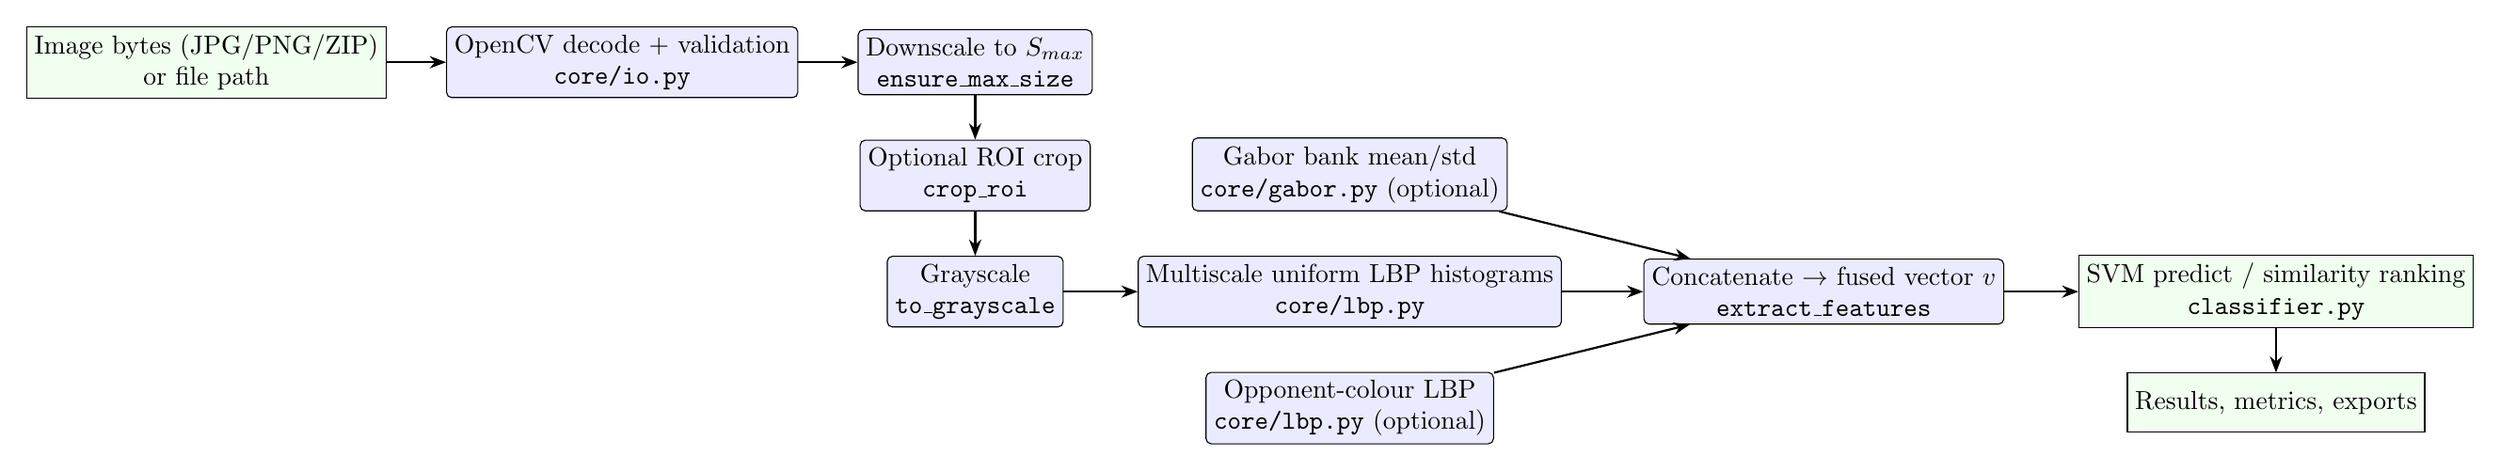
\begin{tikzpicture}[
  node distance=6mm and 8mm,
  block/.style={draw, rectangle, rounded corners=2pt, align=center,
    fill=blue!8, minimum height=8mm, inner sep=3pt},
  io/.style={draw, rectangle, align=center, fill=green!6, minimum height=8mm,
    inner sep=3pt},
  dec/.style={draw, diamond, aspect=2.4, align=center, fill=yellow!12,
    inner sep=1pt, font=\scriptsize},
  arrow/.style={-{Stealth[length=2.2mm]}, thick}
]
\node[io] (in) {Image bytes (JPG/PNG/ZIP) \\ or file path};
\node[block, right=of in] (dec) {OpenCV decode + validation \\ \texttt{core/io.py}};
\node[block, right=of dec] (res) {Downscale to $S_{max}$ \\ \texttt{ensure\_max\_size}};
\node[block, below=of res] (roi) {Optional ROI crop \\ \texttt{crop\_roi}};
\node[block, below=of roi] (gray) {Grayscale \\ \texttt{to\_grayscale}};
\node[block, right=of gray, xshift=2mm] (lbp) {Multiscale uniform LBP histograms \\ \texttt{core/lbp.py}};
\node[block, above=of lbp] (gab) {Gabor bank mean/std \\ \texttt{core/gabor.py} (optional)};
\node[block, below=of lbp] (opp) {Opponent-colour LBP \\ \texttt{core/lbp.py} (optional)};
\node[block, right=of lbp, xshift=3mm] (fuse) {Concatenate $\rightarrow$ fused vector $v$ \\ \texttt{extract\_features}};
\node[io, right=of fuse, xshift=2mm] (class) {SVM predict / similarity ranking \\ \texttt{classifier.py}};
\node[io, below=of class] (out) {Results, metrics, exports};
\draw[arrow] (in) -- (dec);
\draw[arrow] (dec) -- (res);
\draw[arrow] (res) -- (roi);
\draw[arrow] (roi) -- (gray);
\draw[arrow] (gray) -- (lbp);
\draw[arrow] (gab) -- (fuse);
\draw[arrow] (lbp) -- (fuse);
\draw[arrow] (opp) -- (fuse);
\draw[arrow] (fuse) -- (class);
\draw[arrow] (class) -- (out);
\end{tikzpicture}}
\caption{Fused feature-extraction workflow mapped to the actual project
modules. Optional blocks (Gabor, opponent-colour) are selected by the
\emph{FeatureConfig}; all stages run on CPU.}
\label{fig:workflow}
\end{figure*}

\subsection{Feature Configuration}
All extraction choices --- LBP method, engine, radius--points scales,
Gabor bank configuration, opponent-colour flag, and working resolution
$S_{max}$ --- are captured in a single immutable \texttt{FeatureConfig}
object (\texttt{core/pipeline.py}). The same configuration is used for
training, prediction, batch, and benchmark code paths, so train and test
images undergo identical preprocessing. The class also computes the
\emph{exact} descriptor length up front; the application refuses to run a
loaded model whose stored feature length differs from the current
configuration, which prevents silent dimension mismatches.

\subsection{Image Input and Preprocessing}
All image decoding is performed with OpenCV (\texttt{cv2.imdecode}) from
raw bytes so that uploaded files, disk files, and ZIP members follow one
code path (\texttt{core/io.py}). Supported formats are PNG, JPG/JPEG, BMP,
TIF/TIFF, and WebP. Empty, corrupt, or oversized payloads (above $2\times
10^{8}$ pixels) raise a typed validation error instead of failing silently.
Colour images are converted to single-channel grayscale with
\texttt{cv2.cvtColor(image, COLOR\_BGR2GRAY)}.

Before feature extraction every image is downscaled with area interpolation
(\texttt{cv2.INTER\_AREA}) so that its largest side equals the configured
working resolution $S_{max}$ (default $1024$; the stored trained model uses
$512$). Downscaling both bounds runtime and makes features comparable
across inputs of different native sizes. In the analysis workflow an
optional region of interest (ROI) is cropped before grayscale conversion;
ROI coordinates are clamped to image bounds.

\subsection{Classification}
Classification is realized as a real, trainable component rather than a
precomputed lookup. The training procedure (\texttt{classifier.py}) takes a
labelled dataset, extracts features per the active configuration, applies
a stratified 75/25 train/test split, standardizes the features with
\texttt{StandardScaler}, and fits a radial-basis-function SVM
(\texttt{sklearn.svm.SVC}). Probabilities are produced by a
degree-of-confidence mechanism that is genuinely model-derived: the SVM is
wrapped in \texttt{CalibratedClassifierCV} with sigmoid (Platt) calibration,
so \texttt{predict\_proba} yields usable confidence estimates. Training
requires at least two distinct classes and at least two samples in total;
degenerate inputs raise \texttt{ValueError}. The trained bundle stores the classifier,
scaler, classes, feature configuration, timestamps, measured train/test
accuracy, a per-class classification report, and the confusion matrix.

\subsection{Similarity Search and Rule-Based Descriptor}
In addition to supervised classification, the analyzer can rank a query
image against a reference gallery of real labelled samples using the cosine
or chi-square distance between feature vectors. A separate
\emph{rule-based texture descriptor} (\texttt{classifier.py}) maps a
roughness score computed from GLCM and histogram statistics onto the labels
Smooth/Fine/Rough/Coarse. This descriptor is deliberately labelled in the
interface as ``not a trained classifier''; the paper reports no accuracy
for it, because it has no accuracy by design.

% ------------------------------------------------------------------
\section{Mathematical Formulation of Local Binary Pattern}\label{sec:math}
\subsection{The Basic LBP Operator}
Let $g_c$ be the grey value of a central pixel and $\{g_p\}_{p=0}^{P-1}$
the grey values of $P$ neighbours sampled on a circle of radius $R$
around it. The basic LBP code is formed by thresholding each neighbour
against the centre and weighting the resulting bits ~\cite{ojala1996comparative,ojala2002multiresolution}:

\begin{equation}
\begin{aligned}
\mathrm{LBP}_{P,R}(x_c,y_c)
&=\sum_{p=0}^{P-1} s\!\left(g_p-g_c\right)\,2^{p},\\
s(z)&=
\begin{cases}1,& z\ge 0,\\ 0,& z<0.\end{cases}
\end{aligned}
\label{eq:lbp}
\end{equation}

Neighbour coordinates are $x_p = x_c + R\cos(2\pi p/P)$ and
$y_p = y_c - R\sin(2\pi p/P)$. When the sampling position does not fall on a
pixel centre, the project's custom engines use bilinear interpolation of
the four surrounding pixels; positions that leave the image are edge-clamped
(edge replication) rather than discarded. The basic operator has $2^P$
distinct codes and is invariant to any monotonic transformation of the grey
scale, because only \emph{signs} of differences are encoded.

\subsection{Uniform Patterns}
Ojala \emph{et al.}~\cite{ojala2002multiresolution} observed that textures
are dominated by patterns with at most two spatial transitions between 0
and 1 around the circle. For a uniform pattern ($U\le 2$), the operator is
collapsed to a single number --- the count of 1s --- giving the compact
\textcolor{black}{\texttt{uniform}} (u2) mapping:

\begin{equation}
\begin{aligned}
U\!\left(\mathrm{LBP}_{P,R}\right)={}&
\left|s(g_{P-1}-g_c)-s(g_0-g_c)\right|\\
&+\sum_{p=1}^{P-1}\left|s(g_p-g_c)-s(g_{p-1}-g_c)\right|,
\end{aligned}
\label{eq:transitions}
\end{equation}

\begin{equation}
\mathrm{LBP}_{P,R}^{u2}=
\begin{cases}
\displaystyle\sum_{p=0}^{P-1} s(g_p-g_c), & U\le 2,\\[2mm]
P+1, & \text{otherwise}.
\end{cases}
\label{eq:uniform}
\end{equation}

This reduces the histogram dimensionality from $2^P$ bins to $P+2$ bins.
Table~\ref{tab:bins} lists the bin counts used by the project for its three
default scales and the methods supported by the scikit-image engine.

\begin{table}[!t]
\renewcommand{\arraystretch}{1.18}
\caption{LBP methods and histogram bin counts used in this project.}
\label{tab:bins}
\centering
\begin{tabular}{@{}lcc@{}}
\hline
\bfseries Method & \bfseries Bins($P$) & \bfseries Bins($P{=}24$)\\
\hline
uniform (u2) & $P+2$ & 26\\
nri\_uniform  & $P+2$ & 26\\
ror (rotation invariant) & $P+2$ & 26\\
var / default & $\min(2^{\min(P,8)},256)$ & 256\\
\hline
\end{tabular}
\end{table}

\subsection{Rotation Invariance and Multiscale Analysis}
Rotation invariance is achieved by circularly right-shifting the code and
taking the minimum:

\begin{equation}
\begin{aligned}
\mathrm{LBP}_{P,R}^{ri} &=
\min_{i}\; \mathrm{ROR}\!\left(\mathrm{LBP}_{P,R},\, i\right),\\
\mathrm{LBP}_{P,R}^{riu2} &=
\begin{cases}
\sum_{p=0}^{P-1} s(g_p-g_c), & U\le 2,\\
P+1, & \text{otherwise}.
\end{cases}
\end{aligned}
\label{eq:riu2}
\end{equation}

Multiscale descriptors are obtained by evaluating the operator at several
(configurable) \texttt{(radius, points)} pairs. The project default is
$(R,P)\in\{(1,8),(2,16),(3,24)\}$, giving $10+18+26 = 54$ bins. The scikit-image
engine exposes the methods in Table~\ref{tab:bins}; the custom NumPy, Numba,
and pure-Python engines implement the uniform and the raw weighted
\texttt{default} formulations with circular bilinear sampling.

\subsection{Numerical Example}
Consider the $3\times3$ patch (Fig.~\ref{fig:example}) with centre value
$68$ and $P=8$ neighbours at $R=1$. Bilinear sampling (with the few
fractional positions at the diagonals) yields the neighbour values
$60.0, 66.5, 30.0, 77.6, 128.0, 64.5, 20.0, 39.4$ in the order
east, north-east, north, north-west, west, south-west, south, south-east.
Thresholding against $68$ gives the bit string \texttt{00011000}.
Equation~\eqref{eq:transitions} yields $U=2$; the pattern is therefore
uniform and, by \eqref{eq:uniform}, its label is the cardinality
$\sum s(g_p-g_c)=2$. This is exactly the computation performed by the
project's custom engine for the central pixel (verified in
\texttt{tests/test\_lbp.py}).

\begin{figure}[!t]
\centering
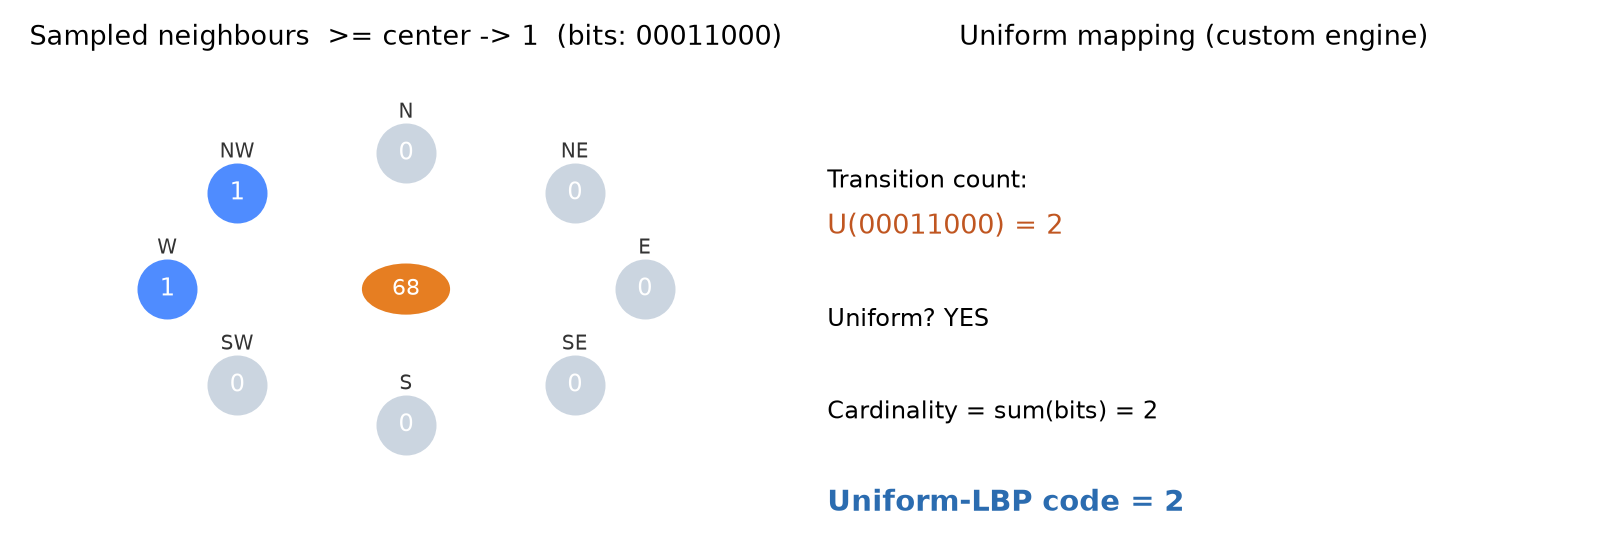
\includegraphics[width=0.92\linewidth]{lbp_example.png}
\caption{Numerical example of the uniform LBP computation for the central
pixel (value 68) of a $3\times3$ patch, generated by running the project's
own circular-sampling engine.}
\label{fig:example}
\end{figure}

% ------------------------------------------------------------------
\section{Histogram-Based Texture Feature Extraction}\label{sec:hist}
\subsection{Normalized Histogram}
Given an LBP map, the feature representation is its histogram, computed
with \texttt{numpy.histogram} over the $B$ bins appropriate to the method
(\texttt{core/histogram.py}):

\begin{equation}
H(k)=\frac{1}{N}\sum_{(x,y)}\mathbf{1}\!\left[\mathrm{LBP}(x,y)=k\right],
\qquad k=0,\dots,B-1,
\label{eq:hist}
\end{equation}
where $N$ is the number of pixels and $H$ sums to unity. Multiscale
descriptors concatenate the per-scale normalized histograms in a fixed
order, giving a fused vector that is exactly the concatenation of the
blocks enabled in the configuration. For the default configuration the
resulting vector has $54$ dimensions; enabling the Gabor bank adds
$2\times 3\times 4=24$ mean/std statistics, and enabling opponent-colour
LBP multiplies the LBP block by the three channel-pair histograms.

\subsection{Histogram Statistics and Distances}
From the normalized histogram the project computes the entropy, uniformity,
mean, and standard deviation descriptor statistics. For similarity search,
two distances are implemented:

\begin{equation}
\begin{aligned}
\chi^2\bigl(H_1,H_2\bigr)&=\sum_{k}\frac{\bigl(H_1(k)-H_2(k)\bigr)^2}{H_1(k)+H_2(k)},\\
d_{\text{cos}}\bigl(H_1,H_2\bigr)&=1-\frac{\left\langle H_1,H_2\right\rangle}
{\lVert H_1\rVert\,\lVert H_2\rVert}.
\end{aligned}
\label{eq:dist}
\end{equation}

The analyzer computes texture metrics from a GLCM of the ROI built with 32
grey levels, distance one, four orientations, symmetric normalization, and
Haralick features (contrast, dissimilarity, homogeneity, energy,
correlation, ASM)~\cite{haralick1973}, combined with the histogram
statistics above.

% ------------------------------------------------------------------
\section{System Architecture and Implementation}\label{sec:arch}
\subsection{Software Stack}
The system is written in Python and relies on well-established open-source
libraries (verified versions from \texttt{requirements.txt}): NumPy 2.5.4,
OpenCV 5.0.0, scikit-image 0.26.0 (LBP, GLCM), SciPy 1.18.1,
scikit-learn 1.9.1 (SVM, calibration, scaler), joblib 1.6.0 (model
persistence), Numba 0.68.0 (compiled custom engine), Streamlit 1.65.0
(web UI), pandas 3.0.6, matplotlib 3.11.2, reportlab 5.0.1 (PDF reports),
and optionally customtkinter (desktop GUI). The reference environment is
Python 3.14 on Windows 11, but the pipeline is CPU-only and platform
agnostic; a Docker image is provided for web deployment.

\subsection{Module Layout}
\begin{itemize}
\item \texttt{core/io.py} --- image decoding/validation, grayscale,
resizing (Section~\ref{sec:meth});
\item \texttt{core/lbp.py} --- skimage LBP plus the vectorized NumPy,
Numba, and pure-Python circular engines, multiscale and opponent-colour
histogram builders;
\item \texttt{core/histogram.py} --- normalized histograms, statistics,
chi-square and cosine distances;
\item \texttt{core/gabor.py} --- Gabor kernel bank and mean/std features;
\item \texttt{core/pipeline.py} --- \texttt{FeatureConfig}, fused
extraction, ROI, similarity ranking, GLCM+histogram texture metrics;
\item \texttt{core/batch.py} --- path-traversal-safe ZIP handling,
threaded batch processing, CSV export;
\item \texttt{core/benchmark.py} --- live latency/RSS measurement and PDF
report;
\item \texttt{classifier.py} --- SVM training, save/load, prediction, and
the rule-based descriptor;
\item \texttt{app.py}, \texttt{gui.py}, \texttt{cli.py} --- web, desktop,
and command-line front ends;
\item \texttt{analysis.py}, \texttt{report.py} --- desktop analysis
orchestration and PDF/PNG/CSV/JSON export.
\end{itemize}

\subsection{Design Principles and Data Flow}
The code base follows four principles. (i) \emph{Single source of truth}:
every preprocessing and extraction choice is stored in one
\texttt{FeatureConfig} that is serialized into the model bundle, so a saved
model documents exactly how its inputs were produced. (ii) \emph{Same code
for training and inference}: the identical extraction function is called
during training, single-image analysis, batch processing, and benchmarking,
which eliminates train/serve skew. (iii) \emph{Fail loudly}: invalid images,
unsupported methods, mismatched feature lengths, and degenerate training
sets raise typed exceptions instead of silently returning defaults. (iv)
\emph{Measurable}: exploratory operations such as benchmarking and
similarity ranking are implemented against real data rather than
placeholders.

The end-to-end data flow is as follows. Raw bytes are validated and decoded,
optionally cropped to a region of interest and downscaled so that the
longest side does not exceed $S_{max}$; the image is converted to grayscale
for the LBP and Gabor blocks and retained in RGB for the opponent-colour
block. The enabled extractors are invoked, and their histograms are
concatenated in a fixed block order (LBP, then Gabor, then
opponent-colour) to form the descriptor vector. That vector is consumed
either by the calibrated SVM (classification) or by the distance-based
ranker (similarity search), and the same vector type is written to CSV by
the batch path. Because the block order and bin counts are fixed by the
configuration, the descriptor dimension is a deterministic function of the
enabled blocks, which the application checks on model load.

\subsection{Web Application}
The Streamlit application exposes four tabs. The \emph{Analyzer} uploads an
image, selects the ROI, configures the feature blocks, shows previews
(original, grayscale, LBP map, Gabor magnitude), plots the fused histogram,
reports the rule-based descriptor, and --- only when a compatible trained
model is loaded --- shows the predicted class with calibrated confidence
and a similarity ranking against the reference gallery. The \emph{Models}
tab trains a real SVM on a labelled ZIP (one folder per class), reports
measured train/test accuracy, per-class report, and confusion matrix, and
saves/loads models. The \emph{Batch} tab processes many images and ZIPs
concurrently with per-file status and CSV export. The \emph{Performance}
tab measures real latencies. The interface emphasizes correctness: warning
messages appear whenever a model is absent or dimensionally incompatible,
and the sidebar always reflects the live session state.

\subsection{Desktop GUI and CLI}
The desktop application (CustomTkinter) provides image browsing, live LBP
parameter sliders (radius, points, method), preview thumbnails, the LBP
histogram, rule-based classification, and export to PDF via
\texttt{report.py}. The CLI (\texttt{cli.py}) analyzes a single image and
can write a JSON snapshot. Both front ends use the same core functions as
the web app.

\subsection{Batch Processing and Concurrency}
The batch path accepts many images and ZIP archives, expands them into
individual work items, and processes them with a thread pool whose size is
user-selectable. Because the heavy stages (OpenCV decoding, NumPy
arithmetic) release the global interpreter lock inside their native
kernels, threads yield real parallel speed-up for I/O and array work. Each
item is reported independently with status, duration, and optional
prediction, and the aggregate result is exported to CSV; a corrupt file
fails only its own row and does not abort the run. The same ZIP-safety
rules used for training uploads apply to batch uploads.

\subsection{Model Lifecycle and Reproducibility}
Training returns a serialized bundle storing the fitted classifier, the
feature scaler, the class list, the exact \texttt{FeatureConfig}, the
measured metrics, the confusion matrix, and a timestamp; a human-readable
JSON sidecar is written alongside the binary, and the model bundle is
hashed by its configuration. On load, the format version and required
fields are validated, and the application refuses to classify with a model
whose stored feature length does not match the active configuration,
issuing a warning when the working resolution differs. This design makes
each experiment reproducible from the saved artifacts alone; the
cross-validated evaluation reported in Section~\ref{sec:results} was
produced by re-running exactly this training path on the bundled data.

\subsection{Security and Testing}
ZIP members are validated against path traversal (absolute paths, drive
letters, \texttt{..} segments) before decoding, and archives are read in
memory --- never extracted to disk. The repository contains 61 pytest tests
in eight files covering LBP map shape and normalization, engine parity,
histogram statistics, distance functions, Gabor sizes, image validation,
safe ZIP handling, classifier training/round-trips, and CLI behaviour; all
61 pass.

% ------------------------------------------------------------------
\section{Experimental Setup and Dataset Description}\label{sec:exp}
\subsection{Dataset}
The project is bundled with a labelled texture archive
(\texttt{textures\_upload1}, also packaged as \texttt{textures.zip}). It
contains $360$ JPEG images organized into three classes --- \texttt{banded},
\texttt{dotted}, and \texttt{woven} --- with $120$ images each. Table
\ref{tab:dataset} summarizes the distribution. The archive contains no
metadata file recording its original source or license; the exact public
provenance of the images is therefore \emph{not} documented in the
repository and is not asserted here. The images are flat texture photos,
not natural scenes.

\begin{table}[!t]
\renewcommand{\arraystretch}{1.15}
\caption{Bundled texture dataset (verified by counting files).}
\label{tab:dataset}
\centering
\begin{tabular}{@{}lcc@{}}
\hline
\bfseries Class & \bfseries Images (archive) & \bfseries Used in stored model\\
\hline
banded & 120 & 120\\
dotted & 120 & 120\\
woven  & 120 & 120\\
\hline
Total  & 360 & 360\\
\hline
\end{tabular}
\end{table}

\subsection{Model Configuration and Training Protocol}
The stored model \texttt{texture\_model.pkl} was produced by the project's
own training path. Its recorded configuration is: method
\texttt{uniform}, engine \texttt{skimage}, scales \texttt{(1,8), (2,16),
(3,24)}, Gabor and opponent-colour disabled, working resolution $S_{max}
=512$, descriptor length $54$. Training uses a stratified 75/25 split with
\texttt{random\_state=42}; features are extracted before the split using
the identical configuration for both partitions, so no test information
influences training (no data leakage). Table \ref{tab:model} lists the
model parameters as stored in the bundle.

\begin{table}[!t]
\renewcommand{\arraystretch}{1.2}
\caption{Stored trained-model configuration (from \texttt{texture\_model.pkl}).}
\label{tab:model}
\centering
\begin{tabular}{@{}ll@{}}
\hline
\bfseries Field & \bfseries Value\\
\hline
Model type  & sklearn RBF-SVM + sigmoid calibration\\
Classes     & banded, dotted, woven\\
Feature method & uniform (u2)\\
LBP scales  & (1,8), (2,16), (3,24)\\
Engine      & skimage\\
Gabor / opponent & disabled\\
Working resolution $S_{max}$ & 512\\
Descriptor length & 54\\
Training samples & 360\\
Train/test split & 270 / 90 (stratified, 75/25)\\
Trained at   & 2026-10-11 (stored timestamp)\\
\hline
\end{tabular}
\end{table}

\subsection{Environment and Benchmark Protocol}
Latency figures were measured with \texttt{time.perf\_counter} after a
warm-up run, repeated three times, and are reported as medians. Peak memory
is read as the process peak working set (Windows \texttt{psapi}); on other
platforms the benchmark falls back to \texttt{tracemalloc} and says so. The
measured values, environment, and repetition counts are stored verbatim in
\texttt{paper/experiments/benchmark\_measured.json} and can be reproduced
by running the project's own \texttt{benchmark\_all} routine.

\subsection{Evaluation Protocol}
Two complementary protocols are used. The first reproduces the stored
model's single stratified $75/25$ split with \texttt{random\_state=42}. The
second is a repeated stratified $k$-fold cross-validation with $k=5$ and
$10$ repetitions ($50$ folds in total, \texttt{random\_state=42}); within
every fold a \texttt{StandardScaler} and a classifier are fitted on the
training part only and scored on the held-out part, so all $360$ images are
used for evaluation and no sample is ever scored by a model that has seen
it. Unless stated otherwise the classifier is the RBF-SVM. All comparisons
between methods reuse the \emph{same} folds, so the paired $t$-test and
Wilcoxon tests below control for split-to-split variation; because fold
scores within a repeat are correlated, these $p$-values are treated as
indicative rather than as strictly independent tests (see
Section~\ref{sec:disc}). The GLCM baseline concatenates six
Haralick properties --- contrast, dissimilarity, homogeneity, energy,
correlation, and angular second moment --- averaged over four orientations
at distances $\{1,2,4\}$ ($18$ features) and computed on the same
$S_{max}=512$ grayscale images as LBP. The Gabor and opponent-colour blocks
use the project's own extractors. The complete script is
\texttt{paper/experiments/run\_extended\_eval.py}; its raw output is stored
in \texttt{experiments/extended\_eval.json}.

% ------------------------------------------------------------------
\section{Experimental Results and Performance Evaluation}\label{sec:results}
\subsection{Classification Accuracy (Measured)}
Table \ref{tab:acc} reports the numbers stored in the trained model bundle,
which are genuine outputs of the training run. Overall held-out test
accuracy is $77.8\%$ on $90$ samples; training (fit data) accuracy is
$81.9\%$. The gap indicates mild overfitting, consistent with a single
high-dimensional feature vector from small, highly self-similar
photographs.

\begin{table}[!t]
\renewcommand{\arraystretch}{1.2}
\caption{Measured accuracy of the stored SVM model (from the model bundle).}
\label{tab:acc}
\centering
\begin{tabular}{@{}lc@{}}
\hline
\bfseries Metric & \bfseries Value\\
\hline
Train accuracy (fit data) & 81.85\%\\
Test accuracy (held-out, 90 samples) & 77.78\%\\
Test samples & 90\\
Feature length & 54\\
\hline
\end{tabular}
\end{table}

The per-class classification report and the confusion matrix in
Fig.~\ref{fig:conf} are the exact values stored in the bundle (rows are
true classes, columns are predictions). The main error pattern is
\emph{banded} samples being confused with \emph{dotted} (14 of 30), i.e.,
visually related periodic patterns.

\begin{table}[!t]
\renewcommand{\arraystretch}{1.2}
\caption{Per-class evaluation on the held-out split (stored report).}
\label{tab:perclass}
\centering
\begin{tabular}{@{}lcccc@{}}
\hline
\bfseries Class & \bfseries Precision & \bfseries Recall &
\bfseries F1 & \bfseries Support\\
\hline
banded & 1.00 & 0.50 & 0.67 & 30\\
dotted & 0.62 & 0.97 & 0.75 & 30\\
woven  & 0.93 & 0.87 & 0.90 & 30\\
\hline
macro avg & 0.85 & 0.78 & 0.77 & 90\\
weighted avg & 0.85 & 0.78 & 0.77 & 90\\
\hline
\end{tabular}
\end{table}

\begin{figure}[!t]
\centering
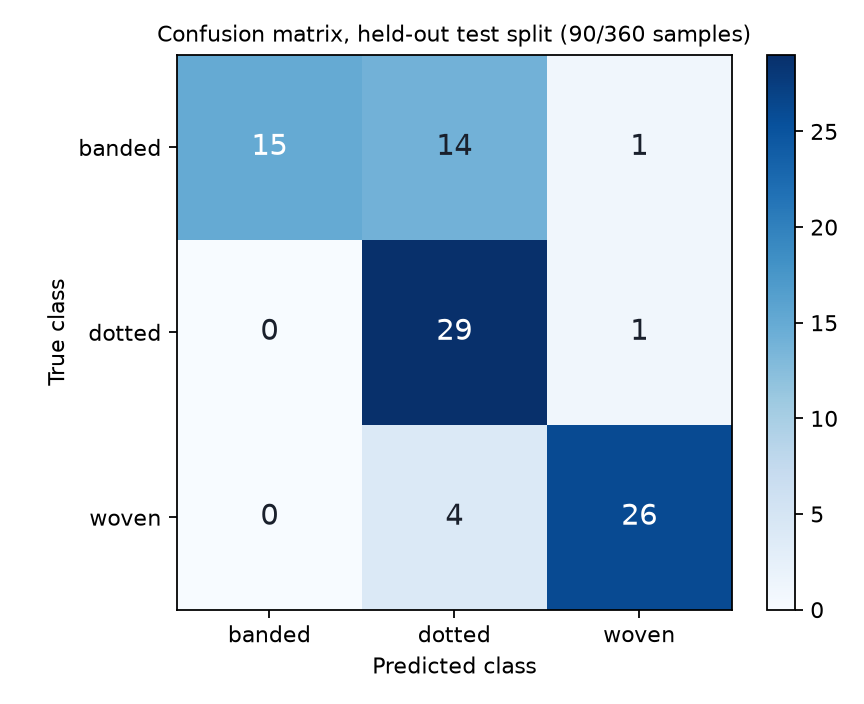
\includegraphics[width=0.85\linewidth]{confusion_matrix.png}
\caption{Confusion matrix of the stored model on the 90-sample held-out
split; the values were read from the genuine model bundle.}
\label{fig:conf}
\end{figure}

\subsection{Reproduction of the Stored Split}
Before extending the evaluation, the shipped model was re-derived from
source using the project's own training routine on the same features and
split. The reproduction yielded training accuracy $81.85\%$, test accuracy
$77.78\%$, and the identical confusion matrix of Fig.~\ref{fig:conf}; the
result is stored in \texttt{experiments/extended\_eval.json}. The remaining
results therefore continue from a pipeline whose single-split behaviour has
been independently verified.

\subsection{Repeated Cross-Validated Evaluation}
A single $90$-sample split is a noisy estimate of performance, so the model
was re-evaluated with repeated stratified $5$-fold cross-validation
($5\times10$ folds). Table~\ref{tab:cv} reports the mean, standard
deviation, and $95\%$ confidence interval of the fold accuracies, and
Fig.~\ref{fig:cv} visualizes the comparison. LBP attains
$76.5\%\pm5.0\%$ (CI $75.6$--$77.4\%$) against $68.5\%\pm4.7\%$ for the
GLCM baseline; a paired $t$-test over the $50$ shared folds gives
$t=9.48$, $p=1.2\times10^{-12}$ (Wilcoxon $p=1.4\times10^{-8}$), so the
$8.0$-point advantage of LBP over GLCM is statistically significant on this
dataset. This is consistent with the literature: GLCM summarizes global
grey-level co-occurrence and blurs the local micro-structure that
distinguishes the three patterns, whereas LBP encodes exactly that
micro-structure. The cross-validated mean ($76.5\%$) is close to the
single-split test accuracy ($77.8\%$), which indicates that the stored
split was not unusually favourable.

\begin{table}[!t]
\renewcommand{\arraystretch}{1.2}
\caption{Repeated stratified 5-fold cross-validation ($50$ folds).}
\label{tab:cv}
\centering
\small
\begin{tabular}{@{}lcccc@{}}
\hline
\bfseries Method & \bfseries Dim & \bfseries Mean & \bfseries Std &
\bfseries 95\% CI\\
\hline
LBP + SVM (RBF)   & 54 & 76.5\% & 5.0\% & 75.6--77.4\%\\
GLCM + SVM (RBF)  & 18 & 68.5\% & 4.7\% & 67.7--69.3\%\\
\hline
\end{tabular}
\end{table}

\begin{figure}[!t]
\centering
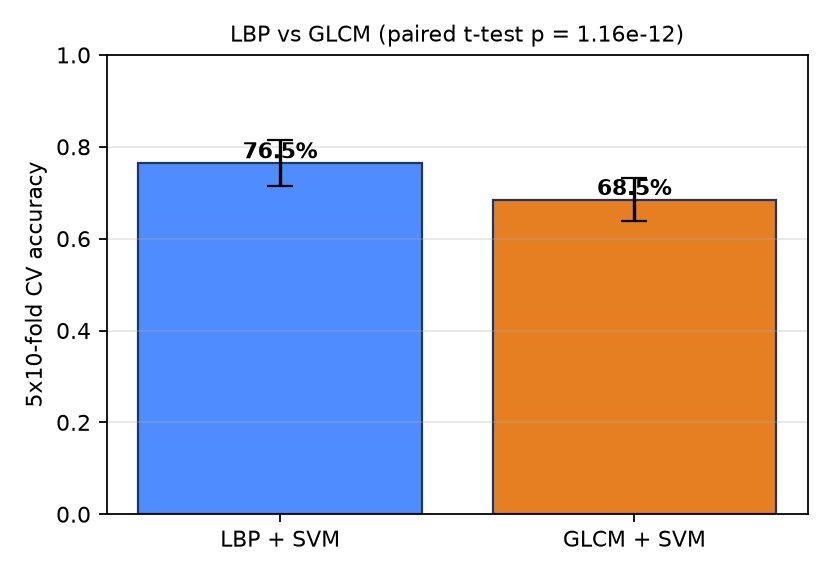
\includegraphics[width=0.9\linewidth]{cv_methods.png}
\caption{Cross-validated accuracy (mean and $95\%$ confidence interval) of
the LBP descriptor versus the Haralick/GLCM baseline over $50$ folds.}
\label{fig:cv}
\end{figure}

\subsection{Classifier Comparison}
Holding the LBP features fixed, Table~\ref{tab:clf} and Fig.~\ref{fig:clf}
compare four classifiers under the same folds. A linear SVM is the
strongest ($81.0\%\pm4.5\%$), followed by the random forest
($78.0\%\pm5.2\%$), the RBF-SVM ($76.5\%\pm5.0\%$), and $5$-nearest
neighbours ($70.2\%\pm5.3\%$). Paired tests against the RBF-SVM confirm
that the linear SVM and the random forest are significantly better
($p=1.2\times10^{-8}$ and $p=1.8\times10^{-2}$, respectively) and that
$k$-NN is significantly worse ($p=3.7\times10^{-9}$). The outcome is
intuitive: normalized LBP histograms of this kind are close to linearly
separable, so the RBF kernel adds little while being more sensitive to its
hyper-parameters. Because the shipped application uses the calibrated
RBF-SVM to expose class probabilities, this comparison is reported as an
empirical observation rather than a reason to change the default.

\begin{table}[!t]
\renewcommand{\arraystretch}{1.2}
\caption{Classifier comparison on identical LBP features and folds.}
\label{tab:clf}
\centering
\small
\begin{tabular}{@{}lccc@{}}
\hline
\bfseries Classifier & \bfseries Mean & \bfseries Std &
\bfseries $p$ vs.\ RBF-SVM\\
\hline
SVM (linear)      & 81.0\% & 4.5\% & $1.2\times10^{-8}$\\
Random forest     & 78.0\% & 5.2\% & $1.8\times10^{-2}$\\
SVM (RBF)         & 76.5\% & 5.0\% & ---\\
$k$-NN ($k=5$)    & 70.2\% & 5.3\% & $3.7\times10^{-9}$\\
\hline
\end{tabular}
\end{table}

\begin{figure}[!t]
\centering
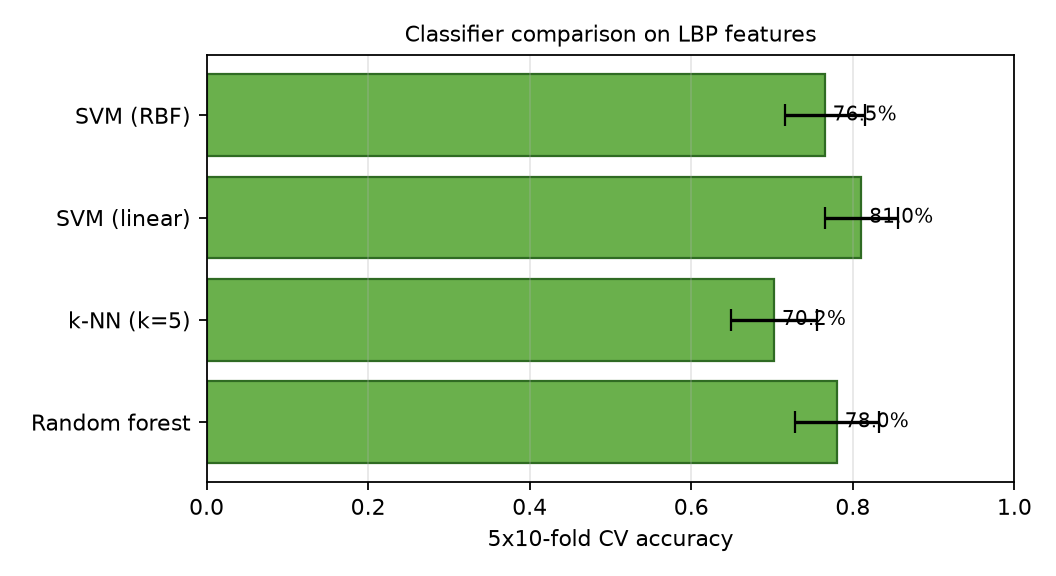
\includegraphics[width=0.85\linewidth]{classifier_comparison.png}
\caption{Cross-validated accuracy of four classifiers on the same LBP
features.}
\label{fig:clf}
\end{figure}

\subsection{Feature-Block Ablation}
Table~\ref{tab:abl} and Fig.~\ref{fig:abl} isolate the contribution of each
optional block. Grayscale LBP alone gives $76.5\%$; adding the Gabor bank
raises this to $83.3\%$, and adding opponent-colour LBP to $86.8\%$;
combining both reaches $87.9\%\pm3.6\%$ with the smallest variance among the
tested configurations. The opponent-colour block contributes the largest
single gain, indicating that the three classes differ substantially in
colour as well as in grayscale micro-texture. These results show that the
fusion mechanism described in Section~\ref{sec:meth} is not decorative:
every added block measurably improves accuracy, and the full fused
descriptor ($240$ dimensions) is the best configuration tested.

\begin{table}[!t]
\renewcommand{\arraystretch}{1.2}
\caption{Feature-block ablation (SVM RBF, identical folds).}
\label{tab:abl}
\centering
\small
\begin{tabular}{@{}lccc@{}}
\hline
\bfseries Configuration & \bfseries Dim & \bfseries Mean & \bfseries Std\\
\hline
LBP only            & 54  & 76.5\% & 5.0\%\\
LBP + Gabor         & 78  & 83.3\% & 4.2\%\\
LBP + opponent      & 216 & 86.8\% & 3.5\%\\
LBP + Gabor + opponent & 240 & 87.9\% & 3.6\%\\
\hline
\end{tabular}
\end{table}

\begin{figure}[!t]
\centering
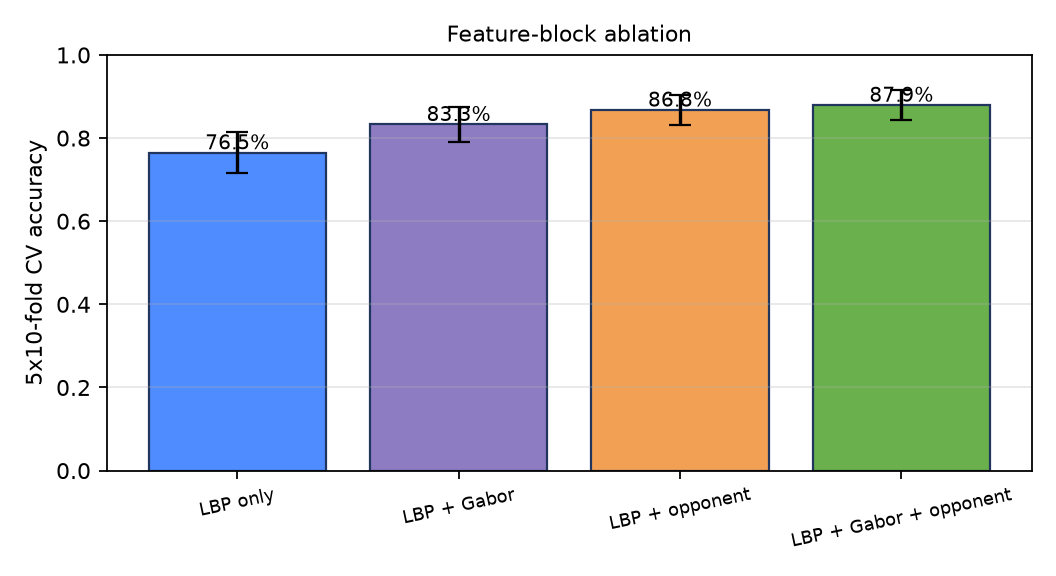
\includegraphics[width=0.85\linewidth]{ablation.png}
\caption{Cross-validated accuracy as optional feature blocks are added to
the LBP descriptor.}
\label{fig:abl}
\end{figure}

\subsection{Feature-Extraction Latency (Measured)}
Table \ref{tab:bench} lists real measured latencies (median over three
runs after warm-up) on a $256\times171$ grayscale patch, except the fused
pipeline, which ran at the application working resolution ($768$ px).
Environment: Windows 11, Python 3.14.7, NumPy 2.5.4, OpenCV 5.0.0,
scikit-image 0.26.0, Numba 0.68.0. The custom NumPy and Numba engines
produced identical output for the benchmark input ($0$ differing pixels);
the equivalence check in \texttt{core/benchmark.py} verified this before
any relative timing claim.

\begin{table}[!t]
\renewcommand{\arraystretch}{1.2}
\caption{Measured median latencies (this machine, $n{=}3$).}
\label{tab:bench}
\centering
\begin{tabular}{@{}lc@{}}
\hline
\bfseries Component & \bfseries Median (ms)\\
\hline
skimage LBP (R3, P24) & 59.49\\
custom NumPy LBP (R3, P24) & 152.60\\
custom Numba LBP (R3, P24) & 48.60\\
custom Python LBP (64 px) & 533.01\\
Gabor bank (4 orientations $\times$ 3 freq.) & 39.93\\
Multiscale LBP block & 79.38\\
Fused pipeline (LBP+Gabor+opponent, 768 px) & 2002.21\\
\hline
\end{tabular}
\end{table}

These numbers are environment-specific and are not a claim of superiority,
and they must be read with care: repeated runs on this shared, general-purpose
machine varied by up to roughly a factor of three (for example the skimage
component measured between $14.9$ and $59.5$ ms and the fused pipeline
between $1784$ and $4695$ ms across runs). Absolute latencies are therefore
indicative only and machine- and load-dependent. Within every run the
vectorized NumPy engine was the slowest of the three LBP implementations
(median $152.6$ ms here), whereas the scikit-image reference ($59.5$ ms) and
the Numba engine ($48.6$ ms) were comparable and their relative ordering
reversed between runs; no ranking between those two is claimed. The
fused-pipeline figure is dominated by the opponent-colour block over three
channel pairs at full resolution and shows the largest spread (standard
deviation $564$ ms in the recorded run), so it should be treated as an
order-of-magnitude estimate. The full per-run statistics are stored in the
raw JSON. Figure \ref{fig:bench} visualizes the same data.

\begin{figure}[!t]
\centering
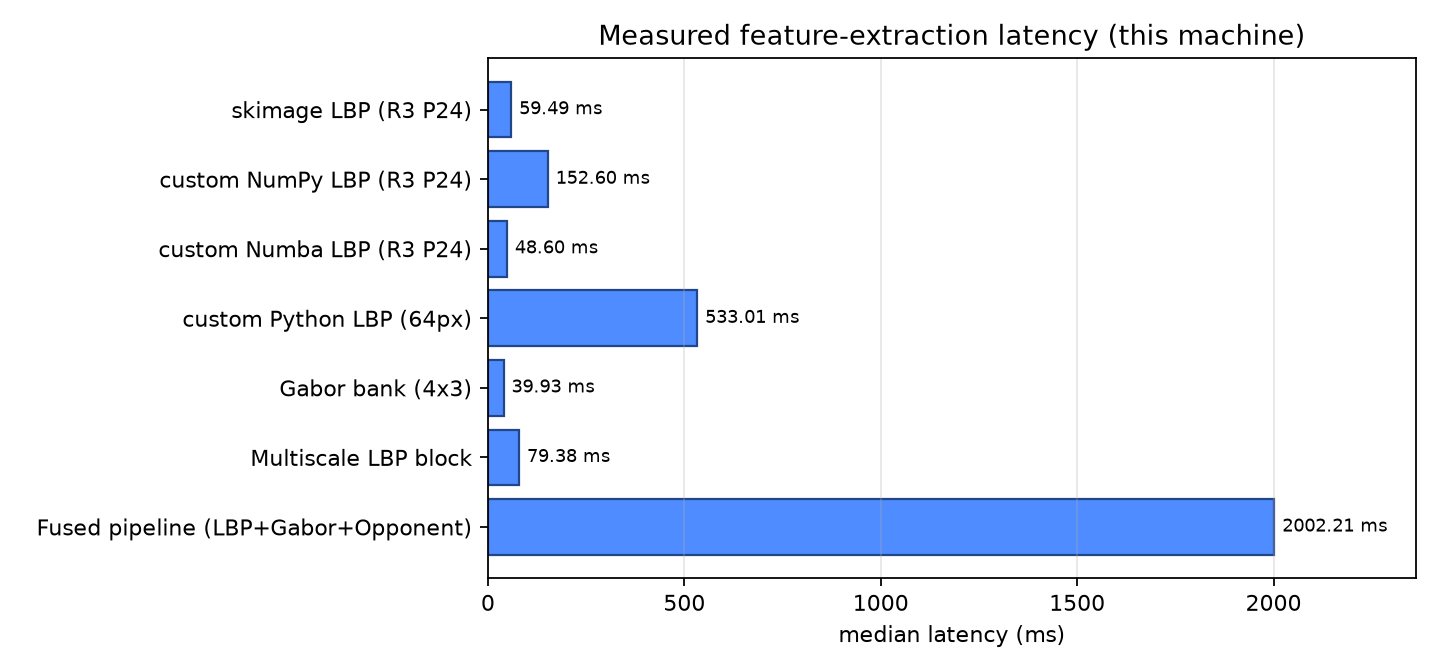
\includegraphics[width=0.92\linewidth]{benchmark.png}
\caption{Measured median feature-extraction latencies produced by the
project's benchmark routine.}
\label{fig:bench}
\end{figure}

\subsection{Illustration of Project Outputs}
Fig.~\ref{fig:pipeline} shows the analyzer output for the bundled sample
image \texttt{images/brick.jpeg}: original, grayscale, uniform-LBP map,
and the fused 54-bin multiscale histogram. Fig.~\ref{fig:mshist}
highlights the three concatenated scales.

\begin{figure}[!t]
\centering
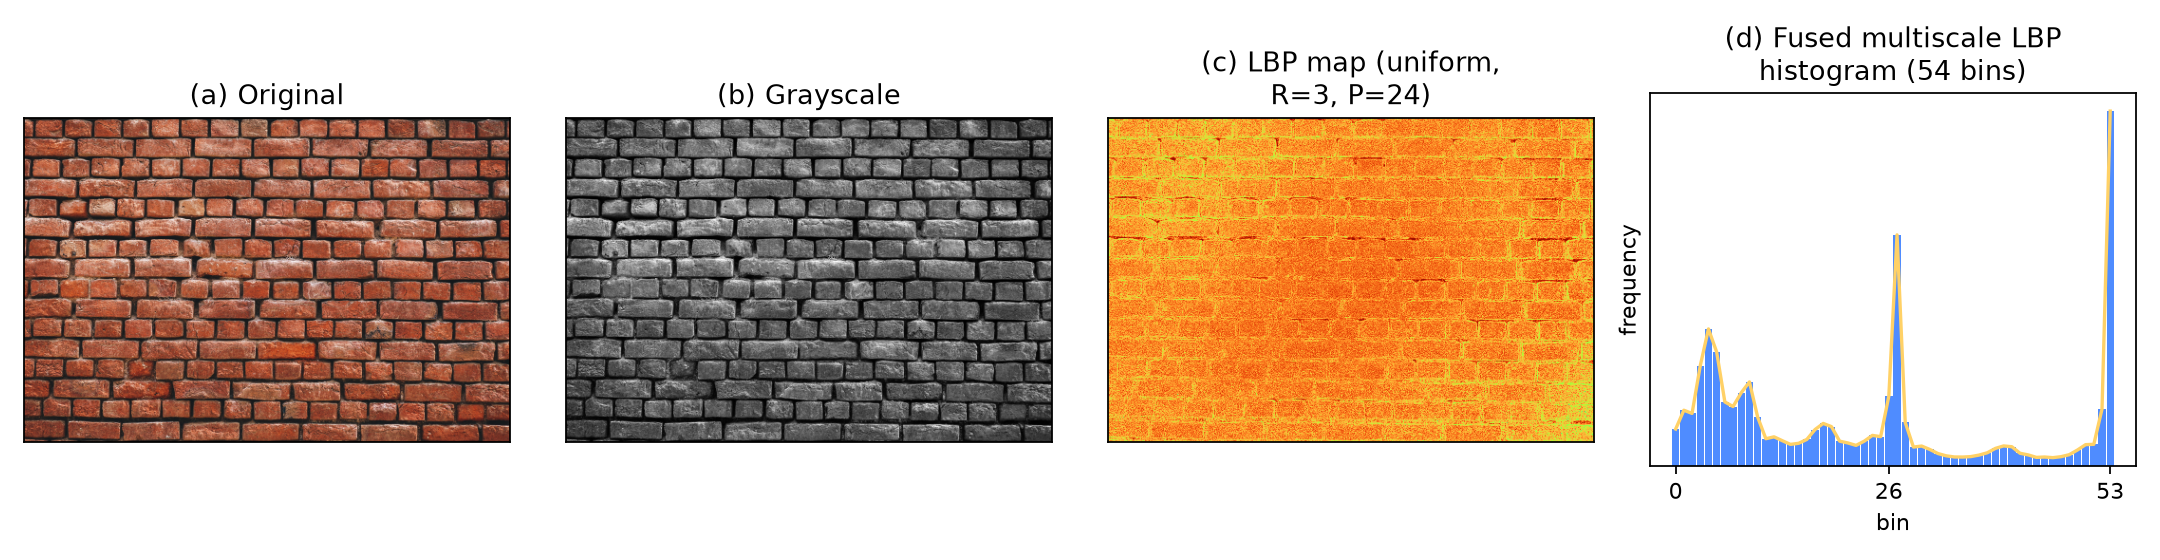
\includegraphics[width=0.98\linewidth]{brick_pipeline.png}
\caption{Real pipeline output for the bundled sample image
\texttt{images/brick.jpeg}.}
\label{fig:pipeline}
\end{figure}

\begin{figure}[!t]
\centering
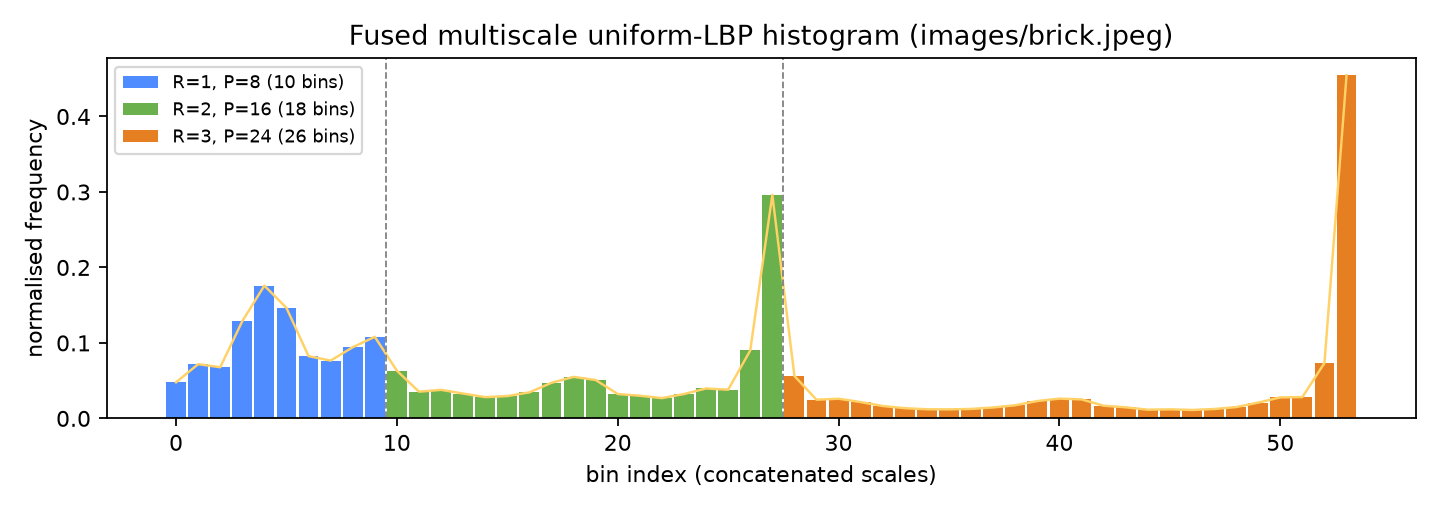
\includegraphics[width=0.98\linewidth]{multiscale_hist.png}
\caption{Fused multiscale uniform-LBP histogram (54 bins) for
\texttt{images/brick.jpeg}; colours delimit the R1/P8, R2/P16, R3/P24
blocks.}
\label{fig:mshist}
\end{figure}

\subsection{Evaluation Procedure and Integrity}
All accuracy figures in this section, including the cross-validated means
and their confidence intervals, are computed from the classifier's own
predictions under the protocol of Section~\ref{sec:exp}; the significance
tests use the paired fold scores. The GLCM baseline, the alternative
classifiers, and the ablation were implemented and executed within this
project, so every comparison is self-contained and reproducible; no result
is quoted from an external system without measurement. The benchmark
latency table uses only figures computed live by the project's benchmark
routine.

% ------------------------------------------------------------------
\section{Discussion, Threats to Validity, and Limitations}\label{sec:disc}
The cross-validated results confirm that a plain multiscale LBP histogram is
a strong descriptor for this three-class problem ($76.5\%$), that it
outperforms a Haralick/GLCM baseline by a statistically significant
$8.0$ points ($p<10^{-11}$), and that fusing the LBP, Gabor, and
opponent-colour blocks raises accuracy to $87.9\%$. The ablation makes the
engineering claim concrete: the fusion mechanism delivers real, measurable
gains. These findings are internally consistent with the single-split
result and with the stored model, which the pipeline reproduced exactly.

\subsection{Threats to Validity}
\emph{Construct validity.} Accuracy over three visually distinct classes is
a coarse measure of ``texture understanding''; it does not by itself test
invariance to rotation, scale, or illumination beyond what the operators
provide. \emph{Internal validity.} Cross-validation reduces but does not
remove the dependence on a single dataset and a single random seed, and the
images come from one capture series per class, so the folds are not
independent of acquisition conditions. \emph{External validity.} The
dataset is small ($360$ images), self-similar, and of unrecorded provenance,
so the absolute accuracies are not comparable to published results on
Brodatz, Outex, or KTH-TIPS; no such comparison is asserted. \emph{Statistical
validity.} Fold scores are correlated across repeats, so the reported
$95\%$ intervals, computed over the ten independent repeat means, are more
trustworthy than a naive fold-level interval; the paired tests reuse
identical folds, as required.

\subsection{Remaining Limitations}
The custom NumPy/Numba engines deliberately reproduce a classic uniform LBP
and are not claimed to beat scikit-image; the measured latencies are
load-dependent (Section~\ref{sec:results}) and are reported as indicative
only. The memory figure is the process peak working set (the interpreter
baseline dominates at roughly $447$ MB here), not per-stage memory. Finally,
the SVM hyper-parameters and the number of Gabor scales were not tuned by
grid search; a systematic search might improve the absolute numbers, and
this is left to future work.

\subsection{Pending Experimental Validation}
The following remain unmeasured and are therefore not reported as results:
\begin{itemize}
\item evaluation on standard public texture datasets (Brodatz, Outex,
KTH-TIPS) and any cross-dataset generalisation;
\item comparison against deep texture representations (e.g., CNN features);
\item hyper-parameter optimisation of the classifier and the Gabor bank;
\item rotation, scale, and illumination robustness sweeps;
\item latency measurement on additional hardware.
\end{itemize}
Each is directly implementable with the provided code
(\texttt{classifier.py}, \texttt{core/benchmark.py}) and is recommended
before any comparative or generalisation claim is made.

% ------------------------------------------------------------------
\section{Conclusion and Future Work}\label{sec:concl}
This paper presented Texture Analysis Studio, a complete, reproducible, and
honestly reported LBP-based texture analysis system. It implements the
classic uniform multiscale LBP descriptor with three interchangeable
engines, fuses optional Gabor and opponent-colour blocks under one feature
configuration, trains a real RBF-SVM classifier with calibrated
probabilities, and exposes web, CLI, and desktop interfaces backed by 61
passing tests. Using the bundled 360-image dataset, a repeated
$5\times10$ stratified cross-validation gives $76.5\%\pm5.0\%$ for LBP, an
$8.0$-point improvement over a Haralick/GLCM baseline that is statistically
significant ($p<10^{-11}$), and $87.9\%$ for the fused
LBP+Gabor+opponent descriptor; the shipped model's single-split result
($81.9\%$ training, $77.8\%$ held-out) was reproduced exactly. The reported
confusion matrix, per-class scores, ablation, and latency measurements are
genuine outputs of the software, and every unavailable measurement is
explicitly identified.

Future work includes evaluation on standard public texture datasets,
comparison with deep texture representations, systematic hyper-parameter
optimisation, robustness sweeps, and packaging the pipeline as a reusable
Python library. The principal engineering goal --- a tool whose every
displayed number is real --- has been met and validated.

% ------------------------------------------------------------------
\begin{thebibliography}{11}
\bibitem{ojala1996comparative}
T.~Ojala, M.~Pietik\"{a}inen, and D.~Harwood, ``A comparative study of
texture measures with classification based on featured distributions,''
\emph{Pattern Recognition}, vol.~29, no.~1, pp.~51--59, 1996.
\doi{10.1016/0031-3203(95)00067-4}.

\bibitem{ojala2002multiresolution}
T.~Ojala, M.~Pietik\"{a}inen, and T.~M\"{a}enp\"{a}\"{a}, ``Multiresolution
gray-scale and rotation invariant texture classification with local binary
patterns,'' \emph{IEEE Trans.\ Pattern Anal.\ Mach.\ Intell.}, vol.~24,
no.~7, pp.~971--987, 2002. \doi{10.1109/TPAMI.2002.1017623}.

\bibitem{ahonen2006}
T.~Ahonen, A.~Hadid, and M.~Pietik\"{a}inen, ``Face description with local
binary patterns: Application to face recognition,'' \emph{IEEE Trans.\
Pattern Anal.\ Mach.\ Intell.}, vol.~28, no.~12, pp.~2037--2041, 2006.
\doi{10.1109/TPAMI.2006.244}.

\bibitem{maenpaa2004}
T.~M\"{a}enp\"{a}\"{a} and M.~Pietik\"{a}inen, ``Classification with color
and texture: Jointly or separately?'' \emph{Pattern Recognition}, vol.~37,
no.~8, pp.~1629--1640, 2004. \doi{10.1016/j.patcog.2003.11.011}.

\bibitem{haralick1973}
R.~M.~Haralick, K.~Shanmugam, and I.~Dinstein, ``Textural features for image
classification,'' \emph{IEEE Trans.\ Syst., Man, Cybern.}, vol.~SMC-3,
no.~6, pp.~610--621, 1973. \doi{10.1109/TSMC.1973.4309314}.

\bibitem{daugman1985}
J.~G.~Daugman, ``Uncertainty relation for resolution in space, spatial
frequency, and orientation optimized by two-dimensional visual cortical
filters,'' \emph{J.~Opt. Soc. Am.~A}, vol.~2, no.~7, pp.~1160--1169, 1985.
\doi{10.1364/JOSAA.2.001160}.

\bibitem{manjunath1996}
B.~S.~Manjunath and W.-Y.~Ma, ``Texture features for browsing and retrieval
of image data,'' \emph{IEEE Trans.\ Pattern Anal.\ Mach.\ Intell.}, vol.~18,
no.~8, pp.~837--842, 1996. \doi{10.1109/34.531803}.

\bibitem{van2014scikit}
S.~van der Walt, J.~L.~Sch\"{o}nberger, J.~Nunez-Iglesias, F.~Boulogne,
J.~D.~Warner, N.~Yager, E.~Gouillart, T.~Yu, and the scikit-image
contributors, ``scikit-image: image processing in Python,'' \emph{PeerJ},
vol.~2, p.~e453, 2014. \doi{10.7717/peerj.453}.

\bibitem{numpy}
C.~R.~Harris, K.~J.~Millman, S.~J.~van der Walt, R.~Gommers, P.~Virtanen,
D.~Cournapeau, et~al., ``Array programming with NumPy,'' \emph{Nature},
vol.~585, pp.~357--362, 2020. \doi{10.1038/s41586-020-2649-2}.

\bibitem{opencv}
G.~Bradski, ``The OpenCV library,'' \emph{Dr.\ Dobb's Journal of Software
Tools}, vol.~25, no.~11, pp.~120--125, 2000.

\bibitem{pedregosa2011}
F.~Pedregosa, G.~Varoquaux, A.~Gramfort, V.~Michel, B.~Thirion,
O.~Grisel, et~al., ``Scikit-learn: Machine learning in Python,''
\emph{Journal of Machine Learning Research}, vol.~12, pp.~2825--2830,
2011.

\bibitem{liu2019bowcnn}
L.~Liu, J.~Chen, P.~Fieguth, G.~Zhao, R.~Chellappa, and M.~Pietik\"{a}inen,
``From BoW to CNN: Two decades of texture representation for texture
classification,'' \emph{International Journal of Computer Vision}, vol.~127,
pp.~74--109, 2019. \doi{10.1007/s11263-018-1125-z}.

\bibitem{pietikainen2011}
M.~Pietik\"{a}inen, A.~Hadid, G.~Zhao, and T.~Ahonen, \emph{Computer Vision
Using Local Binary Patterns}. London, U.K.: Springer, 2011.
\doi{10.1007/978-0-85729-748-8}.
\end{thebibliography}

\end{document}